\documentclass[11pt]{article}
\usepackage{graphicx}

\begin{document}
\title{Lesson 20: Fourier Analysis}
\author{Colt Bradley}
\date{}
\maketitle

\section{Part 1}

\begin{figure}[ht]
\centering
\begin{tabular}{cc}
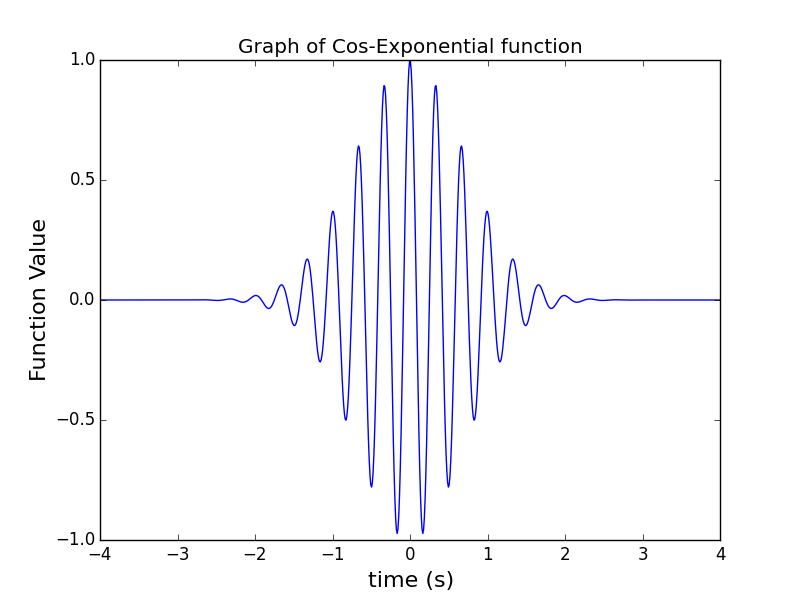
\includegraphics[scale=.4]{cos_wavepacket.png} \\
\multicolumn{2}{c}{(a) $a(t)$ vs time} \\[6pt]

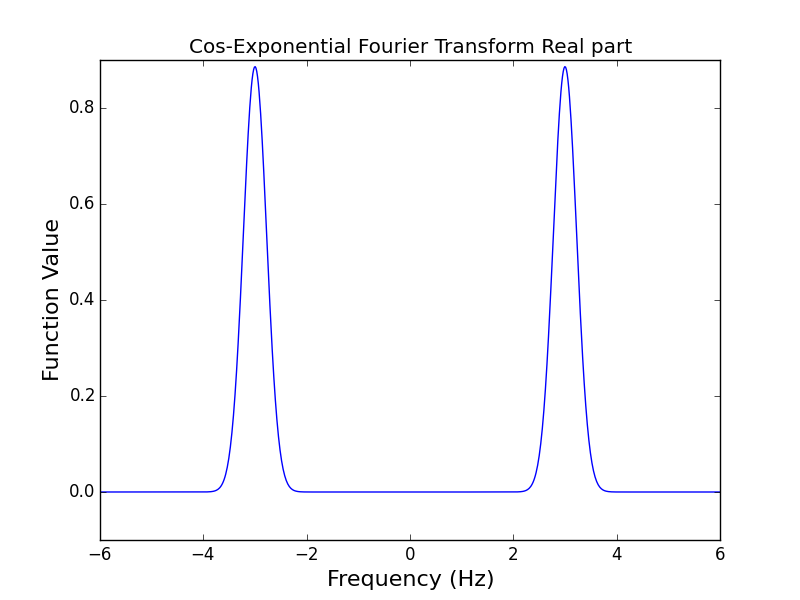
\includegraphics[scale=.4]{cos_fourReal.png}\\
\multicolumn{2}{c}{(b) Real part of $A(f)$ vs frequency} \\[6pt]

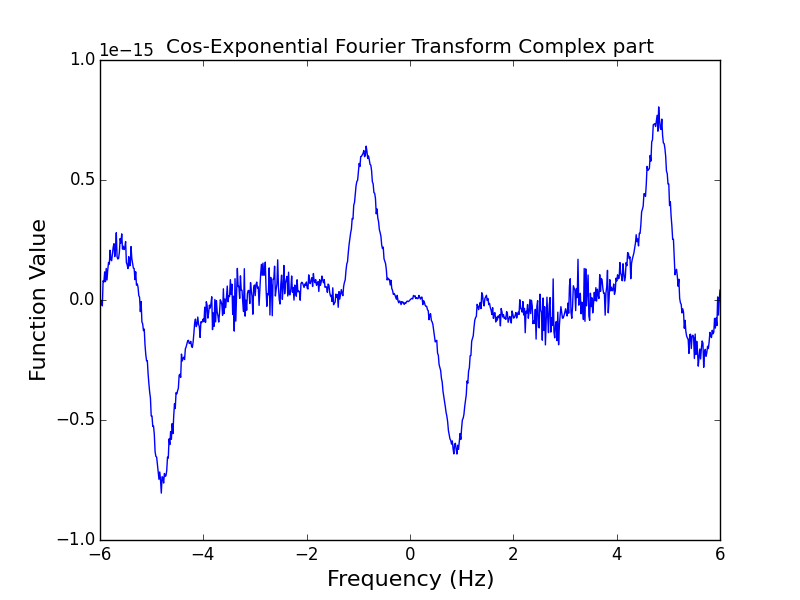
\includegraphics[scale=.4]{cos_fourComp.png}\\
\multicolumn{2}{c}{(c) Complex part of $A(f)$ vs frequency} \\[6pt]
\end{tabular}
\caption{Various plots for $\cos (6\pi t) e^{-t^2} $}
\end{figure}

\begin{figure}[ht]
\centering
\begin{tabular}{cc}
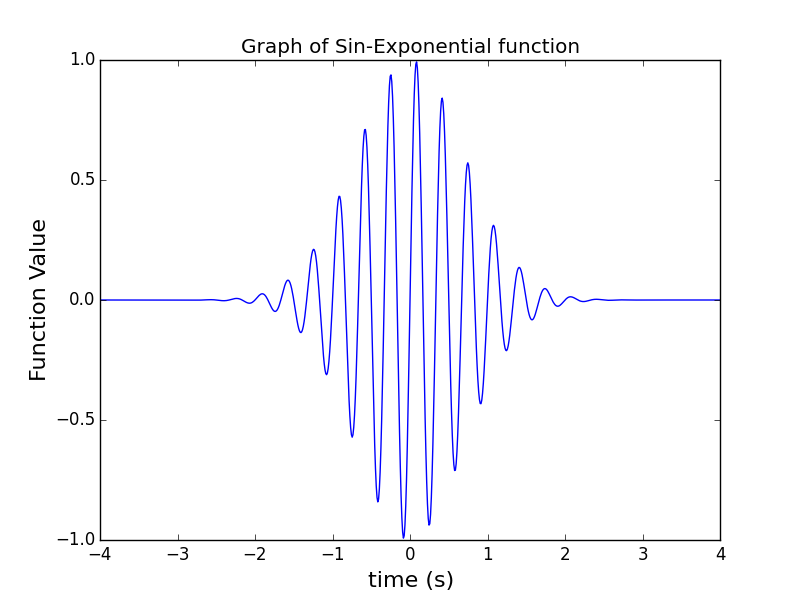
\includegraphics[scale=.4]{sin_wavepacket.png} \\
\multicolumn{2}{c}{(a) $a(t)$ vs time} \\[6pt]

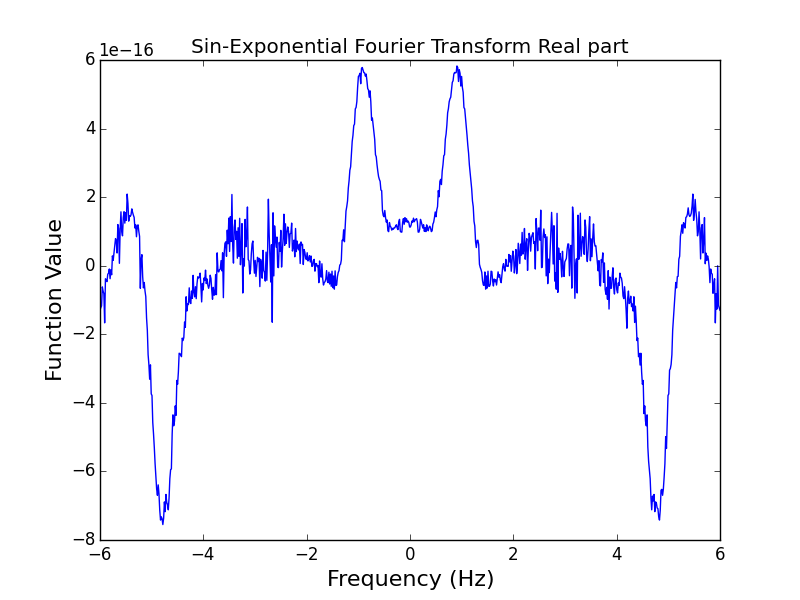
\includegraphics[scale=.4]{sin_fourReal.png}\\
\multicolumn{2}{c}{(b) Real part of $A(f)$ vs frequency} \\[6pt]

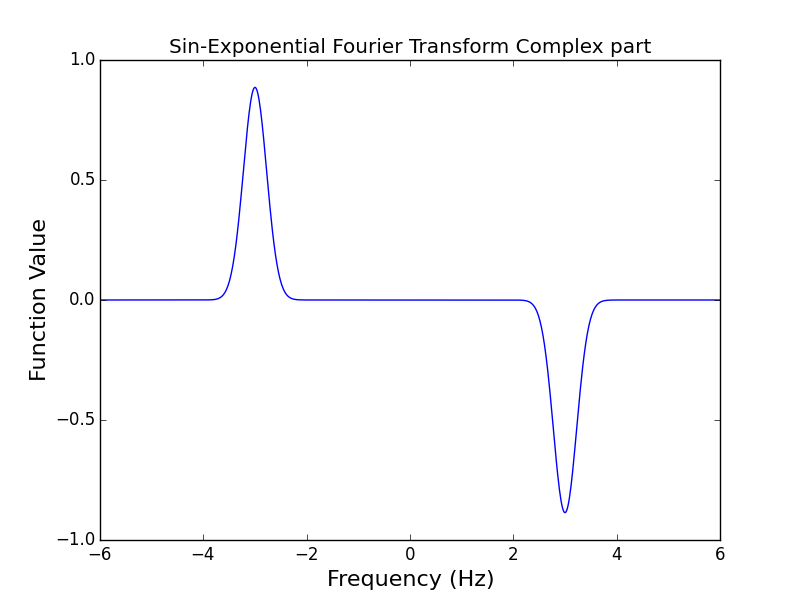
\includegraphics[scale=.4]{sin_fourComp.png}\\
\multicolumn{2}{c}{(c) Complex part of $A(f)$ vs frequency} \\[6pt]
\end{tabular}
\caption{Various plots for $\sin (6\pi t) e^{-t^2} $}
\end{figure}


\section{Part 2}

\begin{figure}[ht]
\centering
\begin{tabular}{cc}
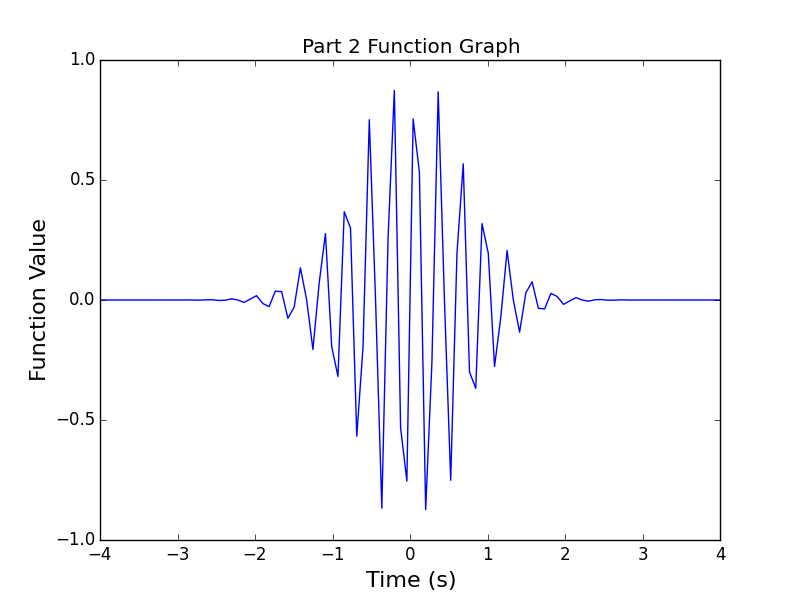
\includegraphics[scale=.4]{prt2_function.png} \\
\multicolumn{2}{c}{(a) $a(t)$ vs time} \\[6pt]

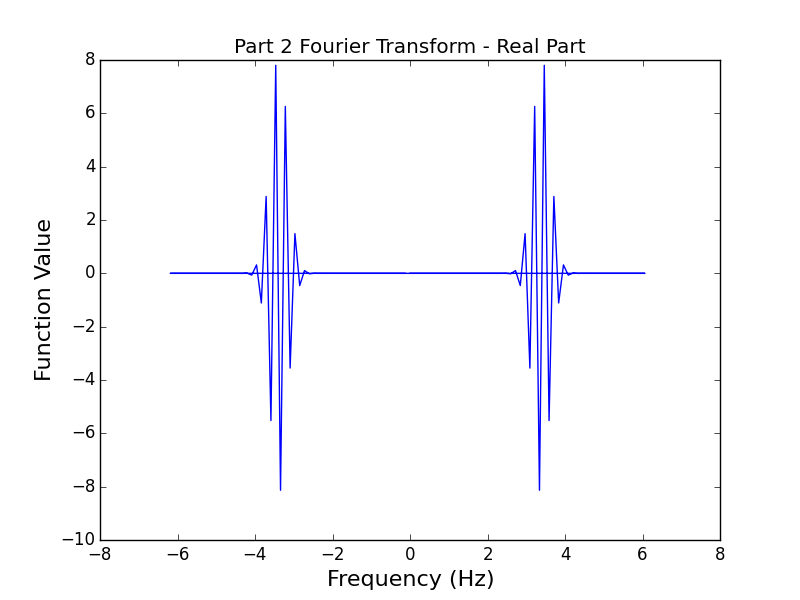
\includegraphics[scale=.4]{prt2_fourReal.png}\\
\multicolumn{2}{c}{(b) Real part of $A(f)$ vs frequency} \\[6pt]

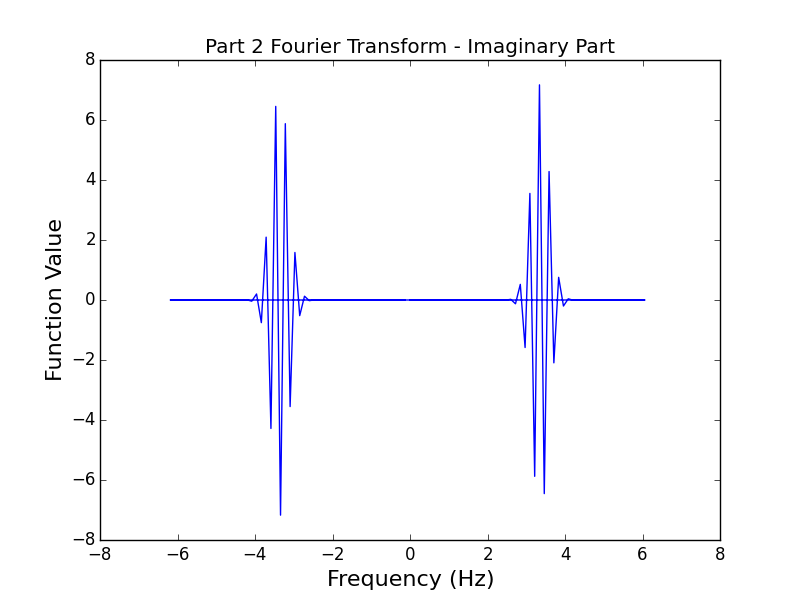
\includegraphics[scale=.4]{prt2_fourComp.png}\\
\multicolumn{2}{c}{(c) Complex part of $A(f)$ vs frequency} \\[6pt]
\end{tabular}
\caption{Various plots for $\cos (6\pi f_0 t) e^{-t^2} $}
\end{figure}

\section{Part 3}

\section{Codes}


\end{document}